\begin{figure}[htbp]
	\centering
	
	\begin{subfigure}{\textwidth}
		\centering
		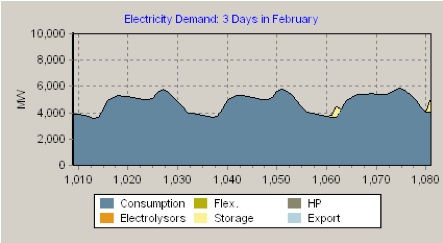
\includegraphics[width=.3\textwidth]{figures/B14-3day-demand.png}\hfill
		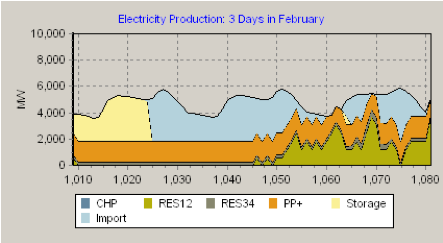
\includegraphics[width=.3\textwidth]{figures/B14-3day-production.png}\hfill
		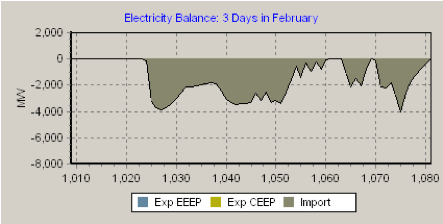
\includegraphics[width=.325\textwidth]{figures/B14-3day-balance.png}
		\caption{Hypothesis with CEEP and MGSPS amendments and no flexible demand}
		\label{fig:B14}
	\end{subfigure}
	
	\vspace{0.25cm}
	
	\begin{subfigure}{\textwidth}
		\centering
		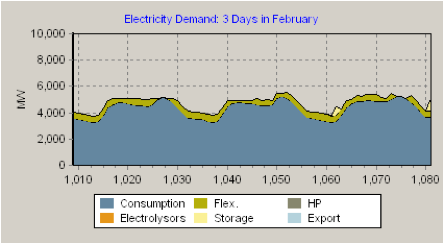
\includegraphics[width=.3\textwidth]{figures/B12-3day-demand.png}\hfill
		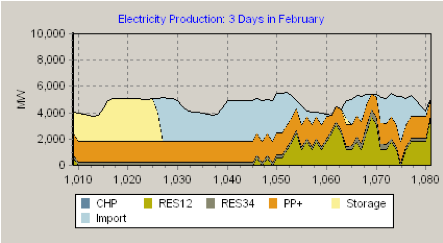
\includegraphics[width=.3\textwidth]{figures/B12-3day-production.png}\hfill
		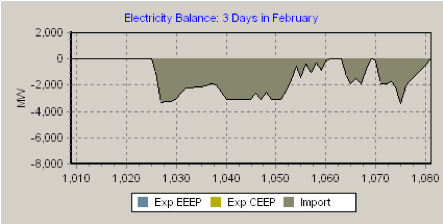
\includegraphics[width=.325\textwidth]{figures/B12-3day-balance.png}
		\caption{Like scenario (a) above but with 10\% flexible demand over one day}
		\label{fig:B12}
	\end{subfigure}
	
	\vspace{0.25cm}
		
	\begin{subfigure}{\textwidth}
		\centering
		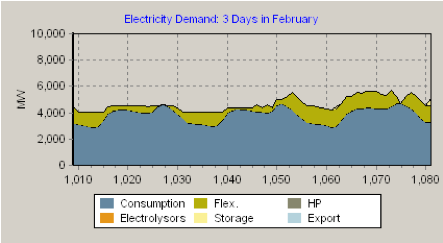
\includegraphics[width=.3\textwidth]{figures/B16-3day-demand.png}\hfill
		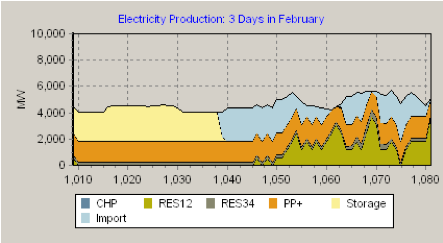
\includegraphics[width=.3\textwidth]{figures/B16-3day-production.png}\hfill
		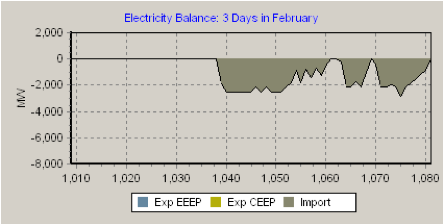
\includegraphics[width=.325\textwidth]{figures/B16-3day-balance.png}
		\caption{Scenario (b) + 10\% flexible demand over one week}
		\label{fig:B16}
	\end{subfigure}
	
	\vspace{0.25cm}
		
	\begin{subfigure}{\textwidth}
		\centering
		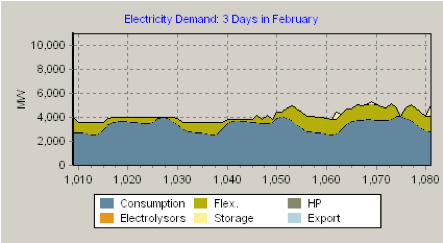
\includegraphics[width=.3\textwidth]{figures/B17-3day-demand.png}\hfill
		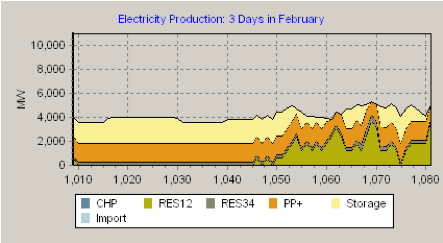
\includegraphics[width=.3\textwidth]{figures/B17-3day-production.png}\hfill
		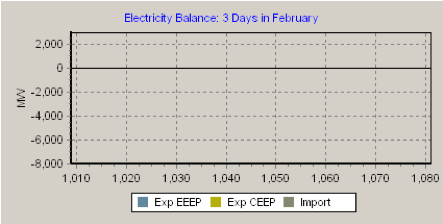
\includegraphics[width=.325\textwidth]{figures/B17-3day-balance.png}
		\caption{Scenario (c) + 10\% flexible demand over four weeks}
		\label{fig:B17}
	\end{subfigure}

	\vspace{0.25cm}

	\rule{\textwidth}{0.5pt} % use line???
	\caption{Graphs showing electricity demand, production and balance in scenarios of increasing flexible demand in EnergyPLAN.}
	\label{fig:flex_dem}
\end{figure}